\documentclass{article}
%% Useful packages
\usepackage[utf8]{inputenc}
\usepackage[a4paper,left=2cm,right=2cm,top=2cm,bottom=2cm]{geometry}
\usepackage{crop,graphicx,amsmath,array,color,amssymb,fancyhdr,lineno}
\usepackage{flushend,stfloats,amsthm,chngpage,times,,lipsum,lastpage} 
\usepackage{calc,listings,color,wrapfig,tabularx,longtable,enumitem}
\usepackage[style=numeric-comp,backend=biber]{biblatex}
\addbibresource{Refs.bib}
\usepackage{lineno}
%%%%%%%%%%%%   Header and Footer  %%%%%%%%%%%%%
\pagestyle{fancy}
\fancypagestyle{plain}{%
  \renewcommand{\headrulewidth}{0pt}%
  \fancyhf{}%
}

\title{%
  First Assignment \\
  \large Equivalent representations of orientation matrices}
\author{Surname Name}

\begin{document}
\begin{titlepage}

\newcommand{\HRule}{\rule{\linewidth}{0.5mm}} % Defines a new command for the horizontal lines, change thickness here

%----------------------------------------------------------------------------------------
%	LOGO SECTION
%----------------------------------------------------------------------------------------
\center

\includegraphics[width=5cm]{Title/Unige-logo.jpeg}\\[1cm] % Include a department/university logo - this will require the graphicx package
 
%----------------------------------------------------------------------------------------

\center % Center everything on the page

%----------------------------------------------------------------------------------------
%	HEADING SECTIONS
%----------------------------------------------------------------------------------------

\textsc{\Huge Università degli studi di Genova}\\[1cm] % Name of your university/college
\textsc{\LARGE DIBRIS}\\[0.3cm]
\textsc{ Department of Computer Science and Technology,}\\
\textsc{ Bioengineering, Robotics and System Engineering}\\[1cm] % Minor heading such as course title
\textsc{\LARGE{Modeling and Control of Manipulators}}\\[1cm] % Major heading such as course name

%----------------------------------------------------------------------------------------
%	TITLE SECTION
%----------------------------------------------------------------------------------------
\makeatletter
\HRule \\[0.4cm]
{ \huge \bfseries Third Assignment}\\[0.2cm] 
{\Large \bfseries Jacobian Matrices and Inverse Kinematics}\\
% Title of your document
\HRule \\[1.5cm]
 
%----------------------------------------------------------------------------------------
%	AUTHOR SECTION
%----------------------------------------------------------------------------------------

\begin{minipage}{0.4\textwidth}
\begin{flushleft} \large
\emph{Author:}\\[0.2cm]
Balia Gian Marco \\
Salterini Filippo \\
Polese Carolina
\\[1.2em]
\emph{Student ID:}\\[0.2cm]
s4398275 \\
s4516129 \\
s4862903 
\\[1.2em]
\end{flushleft}
\end{minipage}
~
\begin{minipage}{0.4\textwidth}
\begin{flushright} \large
\emph{Professors:} \\[0.2cm]
Enrico Simetti\\
Giorgio Cannata  \\[1.2em] % Supervisor's Name

\emph{Tutors:} \\[0.2cm]
Andrea Tiranti\\
Luca Tarasi\\
George Kurshakov
% second marker's name
\end{flushright}
\end{minipage}\\[2cm]
\makeatother

% If you don't want a supervisor, uncomment the two lines below and remove the section above
%\Large \emph{Author:}\\
%John \textsc{Smith}\\[3cm] % Your name

%----------------------------------------------------------------------------------------
%	DATE SECTION
%----------------------------------------------------------------------------------------

{\large \today}\\[2cm] % Date, change the \today to a set date if you want to be precise

\vfill % Fill the rest of the page with whitespace

\end{titlepage}

\sffamily

\fancyhf{}
\fancyhead[L]{Balia Gian Marco - s4398275 \\ Salterini Filippo - s4516129 \\ Polese Carolina - s4862903}
\fancyhead[R]{Modelling and Control of Manipulators - Assignment 3}
\fancyfoot[R]{ \bf\thepage\ \rm }%

\newpage
\tableofcontents

\section*{}
\begin{longtable}{|p{4cm}|p{4cm}|p{4cm}|}
    \hline
    Mathematical expression & Definition & MATLAB expression \\
    \hline 
    $<w>$ & World Coordinate Frame &  w\\[0.4cm]
    $^a_b R$ & Rotation matrix of frame $<b>$ with respect to frame $<a>$  & aRb \\[1.2cm]
    $^a_b T$ & Transformation matrix of frame $<b>$ with respect to frame $<a>$ & aTb \\
    $^a O_b$ & Vector defining frame $<b>$ wit respect to frame $<a>$ & aOb\\
    [1.2cm]
    \hline
    \caption{Nomenclature Table}
\end{longtable}

\section{Assignment description}
The third assignment of Modelling and Control of Manipulators focuses on Inverse Kinematics (IK) control of a robotic manipulator.

The third assignment consists of three exercises. You are asked to:
\begin{itemize}
    \item Download the .zip file called MCM\_assignment3.zip from the Aulaweb page of this course.
    \item Implement the code to solve the exercises on MATLAB by filling in the predefined files. In particular, you will find two different main files: \textit{"ex1.m"} for the first exercise and \textit{"ex2.m"} for the second exercise.
    \item Write a report motivating your answers, following the predefined format on this document.
    \item \textbf{Putting code in the report is not an explanation!}
\end{itemize}

\subsection{Exercise 1}

Given the geometric model of an industrial manipulator used in the previous assignment, you have to add a tool frame.
The tool frame is rigidly attached to the robot end-effector according to the following specifications:  

Use the following specifications
$ {}^e \eta_{t/e}=[0,0,\pi/10], {}^eO_t=[0.2,0,0]^{\top}(cm)$ 
where ${}^e\eta_{t/e}$ represents the YPR values from end effector frame to tool frame.

To complete this task you should modify the class \textit{geometricModel} by adding a new method called \textit{getToolTransformWrtBase}

\subsection{Exercise 2}

Implement an inverse kinematic control loop to control the tool of the manipulator. You should be able to complete this exercise by using the MATLAB classes implemented for the previous assignment (\textit{geometricModel},\textit{kinematicModel}), and also you need to implement a new class \textit{cartesianControl} (see the template attached). The procedure can be split into the following phases

\textbf{Q2.1} Compute the cartesian error between the robot end-effector frame $^b_t T$ and the goal frame $^b_{g} T$.

The goal frame  must be defined knowing that:
\begin{itemize}
    \item The goal position with respect to the base frame is $^b O_g = (-0.14, -0.85, 0.6)^\top(m)$
    \item The goal frame is rotated of $^b \eta_{g} = (-3.02, -0.40, -1.33)^\top(rad)$ around the y-axis of the base frame (inertial frame).
\end{itemize}

\textbf{Q2.2}
Compute the desired angular and linear reference velocities of the end-effector  with respect to the base: $^b \nu^*_{t/0} = \begin{bmatrix}
    \kappa_a &0\\
    0 &\kappa_l
\end{bmatrix}\cdot \begin{bmatrix} \omega^*_{t/0} \\  v^*_{t/0} \end{bmatrix}$, such that $\kappa_{a} = 0.8$,$\kappa_{l} = 0.8$ is the gain.
    
\textbf{Q2.3}
Compute the desired joint velocities $\dot{\bar{q}}$

\textbf{Q2.4}
Simulate the robot motion by implementing the function: \textit{"KinematicSimulation()"} for integrating the joint velocities in time.
\section{Exercise 1} \label{P1}
% Write some intro

From the previous assignment are implemented the same functions \verb*|geometricModel| and \verb*|kinematicModel| with some differences.
In the \verb*|geometricModel| is added a function \verb*|getToolTransformWrtBase| that compute the tool transformation matrix with respect to the base frame $^b_t T = ^b_e T \cdot ^e_t T$. The transformation matrix $^b_e T$ is computed as in the previous assignment with \verb*|getTransformWrtBase|.

\section{Exercise 2}
The Jacobian matrix in \verb*|kinematicModel| due to the presents of the tool is 
\begin{equation} \label{E1}
	^b_t J = ^b \mathbb{S}_{t/e} \cdot ^b J_{e/b}
\end{equation}
where $^b J_{e/b}$ is the basic Jacobian matrix and $^b \mathbb{S}_{t/e} \in \mathbb{R}^{6\times6}$ is the rigid body Jacobian matrix 
\begin{equation*}
	^b \mathbb{S}_{t/e} = \begin{pmatrix}
		I_{3\times 3} & O_{3\times 3}  \\
		[^b \mathbf{r}_{t/e}\times]^\top & I_{3\times 3}
	\end{pmatrix}
\end{equation*}
where $^b \mathbf{r}_{t/e} = ^b \mathbf{r}_{t/b} - ^b \mathbf{r}_{e/b}$.

\subsection{Q2.1}
From $^b \boldsymbol\eta_{g}$ it is computed $^b_g R = ^b_g R_z(\boldsymbol\eta_{g,\mathbf k}) \cdot ^b_g R_y(\boldsymbol\eta_{g,\mathbf j}) \cdot ^b_g R_x(\boldsymbol\eta_{g,\mathbf i})$, checking if it is a proper rotation matrix. Then it is possible to obtain the transformation matrix
\begin{equation*} \renewcommand{\arraystretch}{1.5}
	^b_g T = \begin{pmatrix}
		^b_g R & ^b \mathbf{O}_{g} \\
		\mathbf{O}_{1 \times 3} & 1
	\end{pmatrix}
\end{equation*}
It is implemented the new class \verb*|cartesianControl|, where is present a function \verb*|getCartesianReference| that given the $^b_g T$ computes the Cartesian error.
This function at first compute $^t_g T = {} ^b_t T^{-1} \cdot ^b_g T$, and then obtain $^t\mathbf{h}_{g/t}$ and $\theta$ from $^t_g R$.
The Cartesian error between the robot end-effector frame and the goal frame is
\begin{equation*} \renewcommand{\arraystretch}{1.5}
	^b \mathbf{e}_{t/g} = \begin{pmatrix}
		^b \boldsymbol\rho_{t/g} \\ 
		^b \mathbf{r}_{t/g}
	\end{pmatrix} = \begin{pmatrix}
		^b_t R \cdot ^t\mathbf{h}_{g/t} \cdot \theta \\ 
		^b \mathbf{r}_{g/b} - ^b \mathbf{r}_{t/b}
	\end{pmatrix}
\end{equation*}
where $^b_t R$ is obtained by $^b_t T$ from the Section \ref{P1} with the function \verb*|getTransformWrtBase|.

\subsection{Q2.2}
Desired angular and linear reference velocities of the end-effector  with respect to the base are computed as follow
\begin{equation*}
	^b \boldsymbol\nu^*_{t/0} = \begin{bmatrix}
		\kappa_a &0\\
		0 &\kappa_l
	\end{bmatrix}\cdot 	^b \mathbf{e}_{t/g}
\end{equation*}
where $\kappa_{a} = 0.8$, $\kappa_{l} = 0.8$ are the gain.

\subsection{Q2.3}
The desired joint velocities are computed with the following equation
\begin{equation*}
	\dot{\bar{\mathbf{q}}} = ^b_t J ^\dagger \cdot ^b \boldsymbol\nu^*_{t/0}
\end{equation*}
where $^b_t J ^\dagger$ is the pseudoinverse of the Jacobian matrix computed with the Equation \ref{E1}.

\subsection{Q2.4}
The simulation of the robot's motion is implemented in the function \verb*|KinematicSimulation|. It takes in input: 
\begin{itemize}
	\item the current robot configuration (vector of joint positions) $\mathbf{q}$;
	\item the joints velocity $\dot{\bar{\mathbf{q}}}$;
	\item sample time $t_{s} = \frac{t_{\text{end}} - t_{\text{start}}}{\text{Number of samples}} = 0.1 \,s$;
	\item lower joint bounds $\mathbf{q_{\text{min}}}$;
	\item upper joint bounds $\mathbf{q_{\text{max}}}$.
\end{itemize}
And update $q_{i}$, where $i$ is the $i$-th joint, with the new value $q_{i} + \dot{\bar{q_{i}}} \cdot t_{s}$, if it is not greater of $\mathbf{q_{\text{max}}}$ and lower than $\mathbf{q_{\text{min}}}$. \\
During the simulation the robot's tool moves directly to the goal, see Figure \ref{fig:finalconfiguration} and \ref{fig:motionofthemanipulator}. This is coherent with the graph in Figure \ref{fig:directionvelocitiesee}, indeed both angular and linear velocities are constant, this means that the tool configuration changes constantly (without variation of the velocities).

\begin{figure}
	\centering
	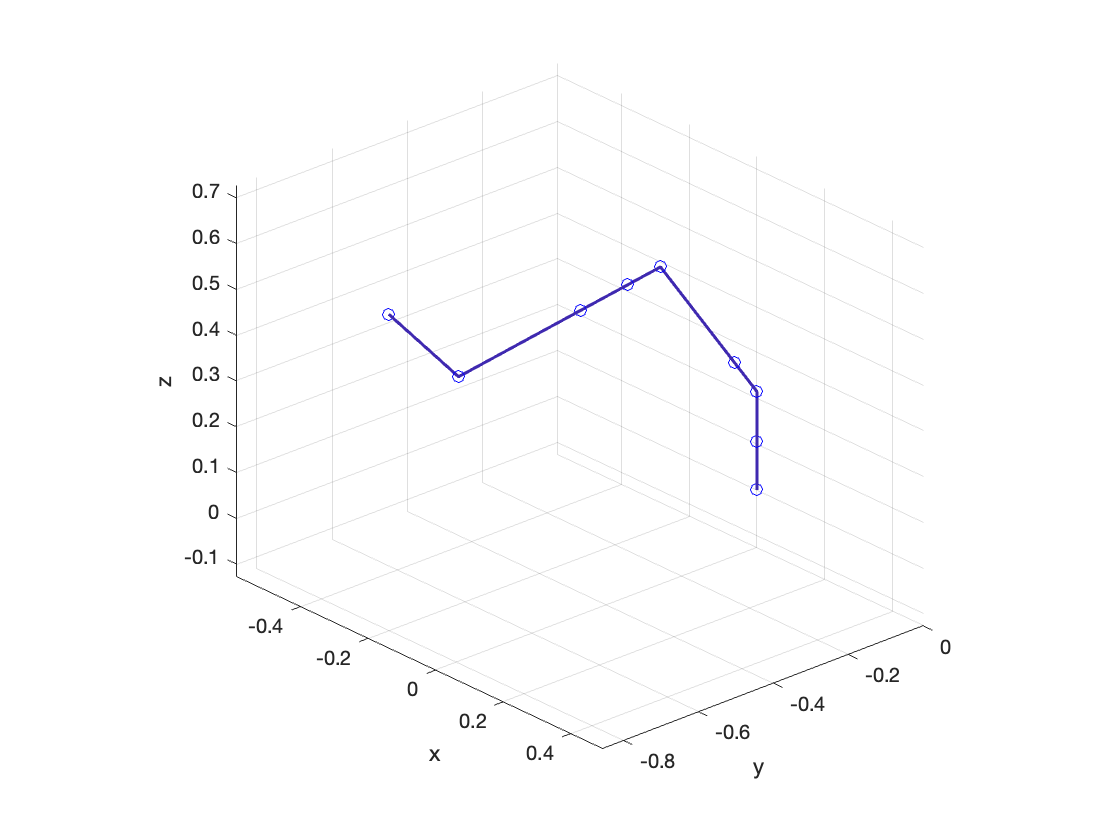
\includegraphics[width=0.7\linewidth]{Resources/FinalConfiguration}
	\caption{Final configuration of the robot during simulated motion in a three-dimensional graph. The measurement units for the three axes are meters.}
	\label{fig:finalconfiguration}
\end{figure}
\begin{figure}
	\centering
	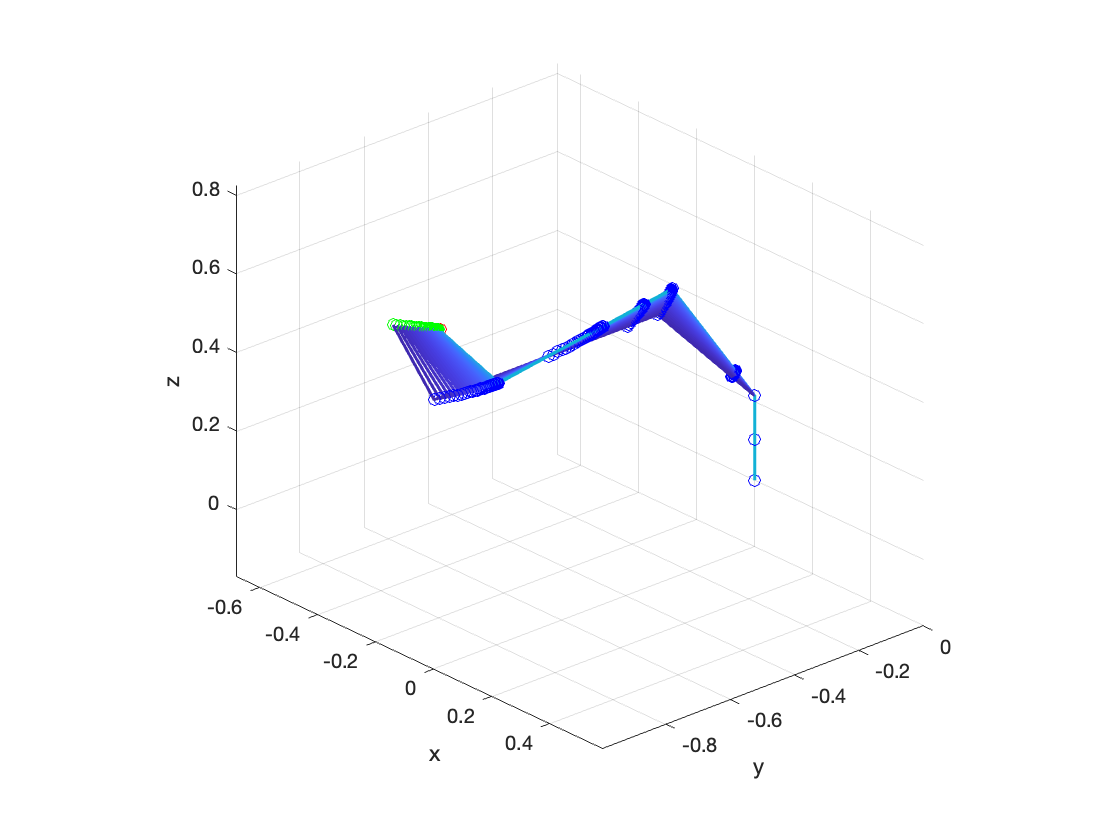
\includegraphics[width=0.7\linewidth]{Resources/MotionOfTheManipulator}
	\caption{ Description of the manipulator’s simulation motion in a three-dimensional graph. The horizontal axes, denoted by x and y, represent the horizontal motion, while the vertical axis, denoted by z, represents the vertical motion. The measurement units for all three axes are meters.}
	\label{fig:motionofthemanipulator}
\end{figure}
\begin{figure}
	\centering
	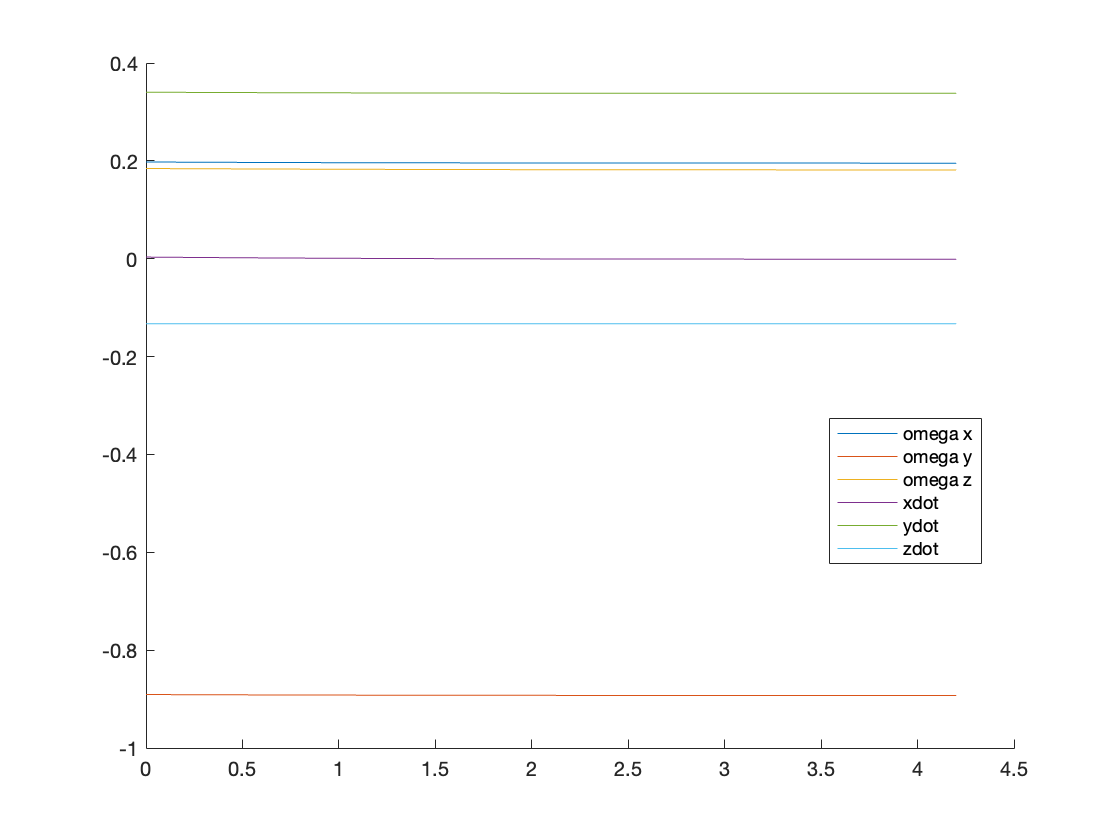
\includegraphics[width=0.7\linewidth]{Resources/DirectionVelocitiesEE}
	\caption{Envelope of end-effector angular ($\frac{rad}{s}$) and linear ($\frac{m}{s}$) velocities' direction.}
	\label{fig:directionvelocitiesee}
\end{figure}


\pagebreak

\section{Appendix}
\textit{[Comment] Add here additional material (if needed)} 
\subsection{Appendix A}

\subsection{Appendix B}


\end{document}
